\chapter{引入预训练模型的联合识别方法}

\section{算法描述}
研究表明,语言模型预训练对于学习通用的语言表示很有用。作为最新的语言模型预训练模型,BERT在许多语言理解任务中均取得了惊人的成绩,
BERT使用双向transformer网络结构来预训练语言模型,着眼于单词左右两侧的上下文,具有更强的表达能力,在大型语料库中训练得到的上下文敏感的语义向量
对语义消歧大有裨益,可以通过附加输出层对bert进行微调来完成模型构建。
在本章,针对跨界服务平台内部数据集有限的现状,我们希望利用bert预训练学到的语义编码能力,来提升第三章中提到的模型的准确率。

\begin{algorithm}
  \caption{引入预训练模型的联合识别}
  \label{alg:suanfa2}
  \begin{algorithmic}[1]
  \Require $L_0$=\{($S_i$,$y_i^d$,$y_i^i$,$y_i^s$)\},i $\in$ [1,n]
  \Ensure $Model_{joint}$\\
模型在训练时,输入的$S_i$为有用户意图的语句,直接将句子中每一个字按照
字向量输入进bert模型编码。模型参数初始化、批处理的数量
iterations = M 和每一批的样本数 batchsize、迭代次数 epoch = N 和当前迭代次数 i = 0\\
\textbf{while} i < N or 模型的性能达到终止条件 \textbf{do}\\
\qquad \qquad \textbf{for} j = 1,\dots ,M \textbf{do}\\
\qquad \qquad \qquad \qquad 随机抽取 batchsize 个训练集数据,前向传输在当前网络权值和输入下网络的输出\\
\qquad \qquad \qquad \qquad 反向传输调整模型参数,对bert参数fine-tuning\\
\qquad \qquad \textbf{end for}\\
\qquad \qquad 计算联合损失 Loss,更新梯度和模型的参数,对bert参数fine-tuning\\
\textbf{end while}\\
用训练好的联合识别模型对测试样本进行预测,计算准确率 Accuracy、损失 Loss
  \State 将用户语句输入神经网络,利用训练好的$Model_{joint}$预测得到与用户意图匹配的服务类型,接口类型和参数信息
  \State 将模型预测的服务,接口,参数等信息传入智能服务调用引擎
  \State 返回服务调用结果
  \end{algorithmic}
  \end{algorithm}

在跨界服务平台中,服务分类,接口分类和参数提取三者具有强相关的特性,对于系统内某一确定的服务,其接口和对应参数的全集也随之确定,
例如对于系统内部的天气服务,其接口仅有query类型,语义槽也是确定的city,date等,因此直觉上可见,可以显示利用任务之间的约束关系来提升模型的性能。
我们尝试了将三者loss函数叠加的隐式联合建模、服务与接口分类向参数提取提供信息流的单向联合识别以及服务分类、接口分类、参数填充三者联系显示建模
的交互式联合识别,以期寻求最优的解决方案,算法描述如算法\ref{alg:suanfa2}。

% \begin{table}[htb]
%   \centering
%   \caption{引入预训练模型的联合识别算法描述}
%   \label{tab:suanfa2}
% \begin{tabular}{p{150mm}}
% \toprule
% \textbf{算法1:}引入预训练模型的联合识别\\
% \textbf{输入:} $L_0$=\{($S_i$,$y_i^d$,$y_i^i$,$y_i^s$)\},i $\in$ [1,n]\\
% \textbf{输出:} $Model_{joint}$\\
% \hline
% \textbf{过程描述:}模型在训练时,输入的$S_i$为有用户意图的语句,直接将句子中每一个字按照
% 字向量输入进bert模型编码。模型参数初始化、批处理的数量
% iterations = M 和每一批的样本数 batchsize、迭代次数 epoch = N 和当前迭代次数 i = 0\\
% \textbf{while} i < N or 模型的性能达到终止条件 \textbf{do}\\
% \qquad \qquad \textbf{for} j = 1,\dots ,M \textbf{do}\\
% \qquad \qquad \qquad \qquad 随机抽取 batchsize 个训练集数据,前向传输在当前网络权值和输入下网络的输出\\
% \qquad \qquad \qquad \qquad 反向传输调整模型参数,对bert参数fine-tuning\\
% \qquad \qquad \textbf{end for}\\
% \qquad \qquad 计算联合损失 Loss,更新梯度和模型的参数,对bert参数fine-tuning\\
% \textbf{end while}\\
% 用训练好的联合识别模型对测试样本进行预测,计算准确率 Accuracy、损失 Loss\\
% \bottomrule
% \end{tabular}
% \end{table}


\section{服务分类、接口分类与参数填充联合识别}
\subsection{slot-oriented联合识别}
如上小节所述,参数提取任务和服务分类、接口分类任务之间存在很强的关联性,而第三章的pipeline方法是三项任务各自独立,未能考虑到任务之间的关联性。
而建立联合损失函数的方法“隐式”考量了三个任务之间的联系,但并未明确为服务分类、
接口分类和服务参数填充之间进行显示的关联建模,考虑到由于服务参数填充通常高度依赖于前两个任务,
因此本节进行了单向联合识别的尝试,提出了单向联合模型,以期通过整合全局信息流方向来优化获得更好的语义理解结果。
同时,和上一章一样,注意力机制被引入到模型中,在编码时提供精确的关注焦点。
本节的模型着重于介绍如何通过引入参数提取门控机制来对服务分类,接口分类和服务参数填充之间进行显式关系建模。


如图\ref{fig:lianhe1}所示,设slot-oriented联合识别模型输入的词序列是x=[$x_{1}$,$x_{2}$,\dots,$x_{T}$],$x_{i}$经过双向LSTM处理后
得到的结果是$\overleftarrow{\mathbf{h}}_{i}$和$\overrightarrow{\mathbf{h}}_{i}$,
拼接以后在第i步得到的结果是$\mathbf{h}_{i}=[\overrightarrow{\mathbf{h}}_{i} ;\overleftarrow{\mathbf{h}}_{i}]$。

(1)attention层

我们在联合模型中共设置了三层注意力机制,分别用于服务分类、接口分类与参数填充,三者的attention原理相同,只是会训练各自的参数,因此可以合并介绍。
设BLSTM得到的隐层向量序列为$h_{1}$,$h_{2}$,\dots,$h_{T}$,我们引入上下文向量${c}_{i}$来表示经过attention权重$α_{i,j}$和处理后的BLSTM隐层向量,
具体的${c}_{i}^{D}$,${c}_{i}^{I}$,${c}_{i}^{S}$分别表示用于服务分类、接口分类与参数填充任务的上下文向量:
\begin{equation}
    \mathbf{c}_{i}=\sum_{j=1}^{T} \alpha_{i, j} \mathbf{h}_{j}
  \end{equation}
  其中$\alpha_{i, j}$也根据所在具体的attention层不同分为$\alpha_{i, j}^{D}$,$\alpha_{i, j}^{I}$,$\alpha_{i, j}^{S}$,计算公式如下:
  \begin{equation}
    \alpha_{t, j}=\frac{\exp \left(\operatorname{score}\left(\mathbf{h}_{i}, \mathbf{h}_{j}\right)\right)}{\sum_{k} \exp \left(\operatorname{score}\left(\mathbf{h}_{i}, \mathbf{x}_{k}\right)\right)}
    \end{equation}
    \begin{equation}
      \operatorname{score}(\mathbf{h}_{i}, \mathbf{h}_{j}))=\tanh \left(\mathbf{W}\left[\mathbf{h}_{i} ; \mathbf{h}_{j}\right]\right)
    \end{equation}
显然这里的$\mathbf{W}$可根据任务具体分为$\mathbf{W}_D$,$\mathbf{W}_I$,$\mathbf{W}_S$

\begin{figure}[htbp]
  \centering
  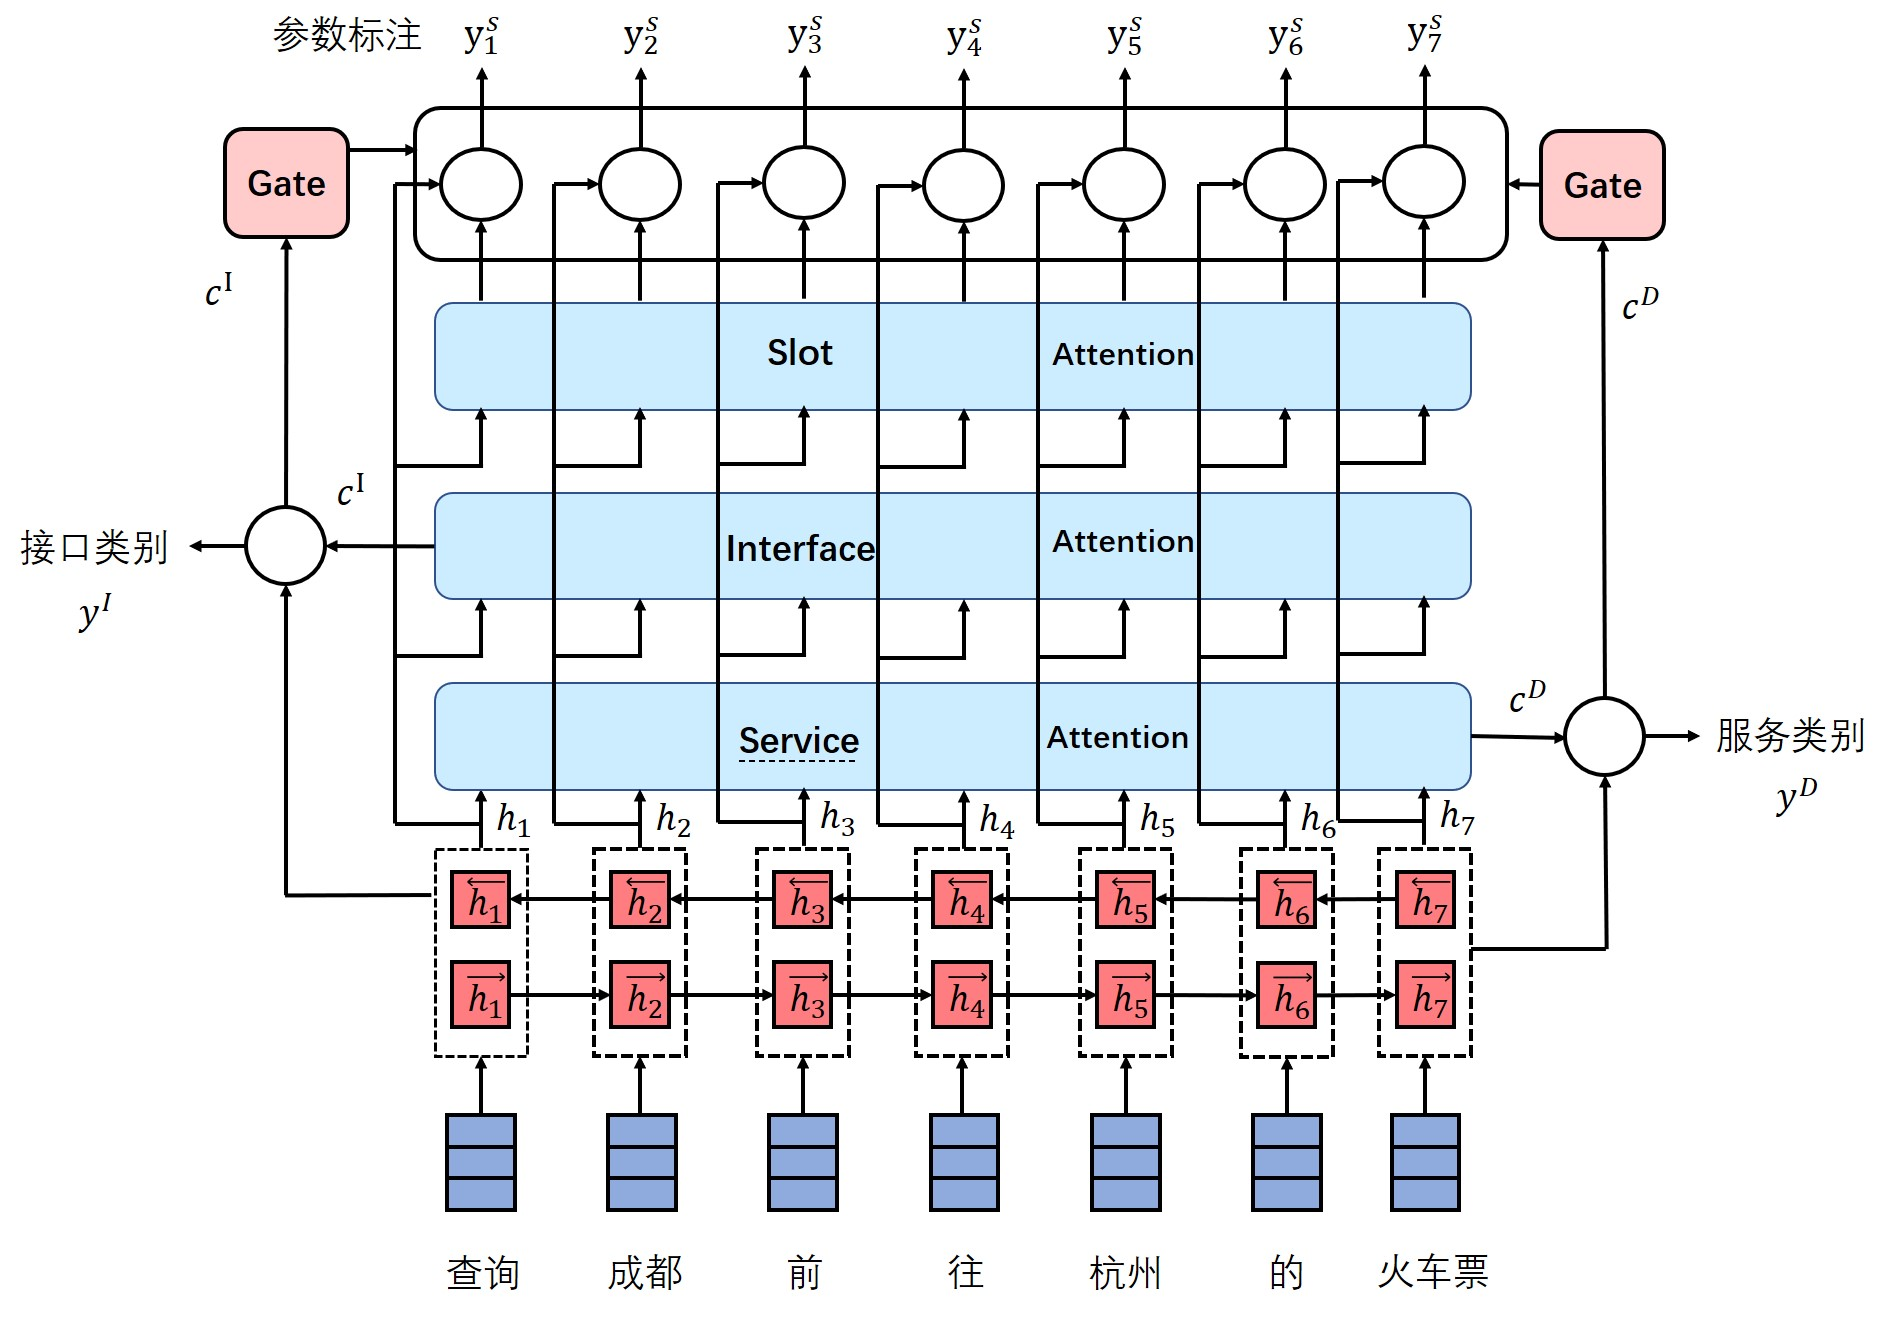
\includegraphics[width=17cm]{./images/lianhe.jpg}
  \caption{slot-oriented联合识别模型}
  \label{fig:lianhe1}
\end{figure}

(2)服务分类

我们以(1)中计算服务分类上下文向量的方法可以得到${c}_{i}^{D}$,再从BLSTM中取$\overleftarrow{\mathbf{h}}_{1}$和$\overrightarrow{\mathbf{h}}_{T}$,
$c^{D}$表示所有步骤得到的$c_i^{D}$的均值,服务的类别预测可由下式得到:
\begin{equation}
    y^{D}=\operatorname{softmax}\left(W^{D}\left(\overleftarrow{\mathbf{h}}_{1}+\overrightarrow{\mathbf{h}}_{T}+c^{D}\right)\right)
  \end{equation}
  \begin{equation}
    c^{D}=\frac{1}{T}\sum_{i=1}^{T} c_i^{D}
  \end{equation}

(3)接口分类

  我们以(1)中计算接口分类上下文向量的方法可以得到${c}_{i}^{D}$,再从BLSTM中取$\overleftarrow{\mathbf{h}}_{1}$和$\overrightarrow{\mathbf{h}}_{T}$,
  $c^{I}$表示所有步骤得到的$c_i^{I}$的均值,接口的类别预测可由下式得到:
  \begin{equation}
      y^{I}=\operatorname{softmax}\left(W^{I}\left(\overleftarrow{\mathbf{h}}_{1}+\overrightarrow{\mathbf{h}}_{T}+c^{I}\right)\right)
    \end{equation} 
    \begin{equation}
        c^{I}=\frac{1}{T}\sum_{i=1}^{T} c_i^{I}
      \end{equation}


(4)参数提取

如图\ref{fig:gate}中的gate,我们引入参数提取的控制门利用服务类型上下文向量${c}_{i}^{D}$和接口类型上下文向量${c}_{i}^{I}$来建模服务、接口与参数填充的关系
以期提高参数提取的准确率。${c}^{D}$,${c}^{I}$,${c}_{i}^{S}$会在每一个步长传入gate结构中计算:
\begin{equation}
    g=\sum v \cdot \tanh (c_{i}^{S}+W_D \cdot c^{D}+W_I \cdot c^{I})
  \end{equation}
其中$\mathbf{v},\mathbf{W}_D,\mathbf{W}_I$是可训练的参数,数值g可以被看作联合上下文向量${c}^{D}$,${c}^{I}$,${c}_{i}^{S}$计算得到的权值,
较大的g表示slot上下文向量和D、I上下文向量“注意力一致”,可以推断出该语义槽和服务、接口之间的相关性更强,该词更有可能是我们需要提取的参数。
最终第i个词的标签类别信息可由下式计算得出:
\begin{equation}
    y_{i}^{S}=\operatorname{softmax}\left(W_{h y}^{S}\left(h_{i}+c_{i}^{S} \cdot g\right)\right)
  \end{equation}

  \begin{figure}[htbp]
    \centering
    
\includegraphics[scale=0.3]{./images/gate.jpg}
    \caption{gate结构}
    \label{fig:gate}
  \end{figure}

(5)联合目标函数

为了同时完成服务分类、接口分类与参数填充三项任务,需要建立联合损失函数,假设$y^D,y^I,y^S$表示正确的类别与标注,我们的目标
便是使在输入为$\mathbf{x}$的条件下概率$p\left(y^{S}, y^{I},y^{D} \mid \mathbf{x}\right)$最大:
\begin{equation}
    \begin{array}{l}
        p\left(y^{S}, y^{I},y^{D} \mid \mathbf{x}\right) \\
        =p\left(y^{D} \mid \mathbf{x}\right) p\left(y^{I} \mid \mathbf{x}\right) \prod_{t=1}^{T} p\left(y_{t}^{S} \mid \mathbf{x}\right) \\
        =p(y^{D} \mid x_{1}, \ldots, x_{T}) p(y^{I} \mid x_{1}, \ldots, x_{T}) \prod_{t=1}^{T} p(y_{t}^{S} \mid x_{1}, \ldots, x_{T})
        \end{array}
    \end{equation}

\subsection{co-interactive联合识别}
上一个的模型完成了从各任务独自建模到服务分类、接口分类向参数填充传递信息流的转换,
但只考虑了从服务和接口到参数填充的单向信息流,而忽略了显式应用参数填充(语义槽)信息来指导前两项任务,这导致无法有效地建立双向连接。
直观的讲,如果用户的意图是调用平台内部的火车票查询服务,他输入的语句更可能出现诸如起始终点城市,日期等语义槽;反之,如果一句话中包含了
出发的起始,目的地和日期,那用户的意图更可能是调用行程相关的服务。因此,考虑任务与任务之间的交互影响十分重要\ref{fig:lianhe2}。

在本模型中,核心组件是协同交互层模块,用于对任务与任务之间关系的显示建模,旨在考虑任务与任务的交叉影响以及相互促进。
具体来说,在协同交互层模块中,
我们首先在服务、接口和参数填充分别应用注意力机制,以捕获初始的显式向量表示,从而提取三个任务的语义信息。
其次,将明确的服务、接口和参数填充表示形式馈入一个共同交互的注意层,以进行信息流的多向充分融合。
将服务分类向量视为查询$Q_D$,参数填充向量视为键$K_S$以及值$K_S$,以获取可感知服务分类信息的参数填充向量表示信息并反馈给服务分类任务;
接口分类向量视为键$K_I$以及值$K_I$,以获取可感知服务分类信息的接口向量表示信息并反馈给服务分类任务。
将接口分类向量视为查询$Q_I$,参数填充向量视为键$K_S$以及值$K_S$,以获取可感知接口分类信息的参数填充向量表示信息并反馈给接口分类任务;
服务分类向量视为键$K_D$以及值$K_D$,以获取可感知接口分类信息的服务向量表示信息并反馈给接口分类任务。
将参数填充向量视为查询$Q_S$,服务分类向量视为键$K_D$以及值$K_D$,以获取可感知参数填充信息的服务分类向量表示信息并反馈给参数填充任务;
接口分类向量视为键$K_I$以及值$K_I$,以获取可感知参数填充信息的接口向量表示信息并反馈给参数填充任务。
基于此操作,可以建立多个任务之间的显示连接,背后的原理是通过协同互动的注意力机制获取相应的交互信息。
参考transformer的设计,可以将协同交互模块堆叠在一起以形成一个层次结构,该层次结构使任务之间能够进行多次交互,从而实现增量捕获交互信息来达到彼此丰富。

\begin{figure}[htbp]
  \centering
  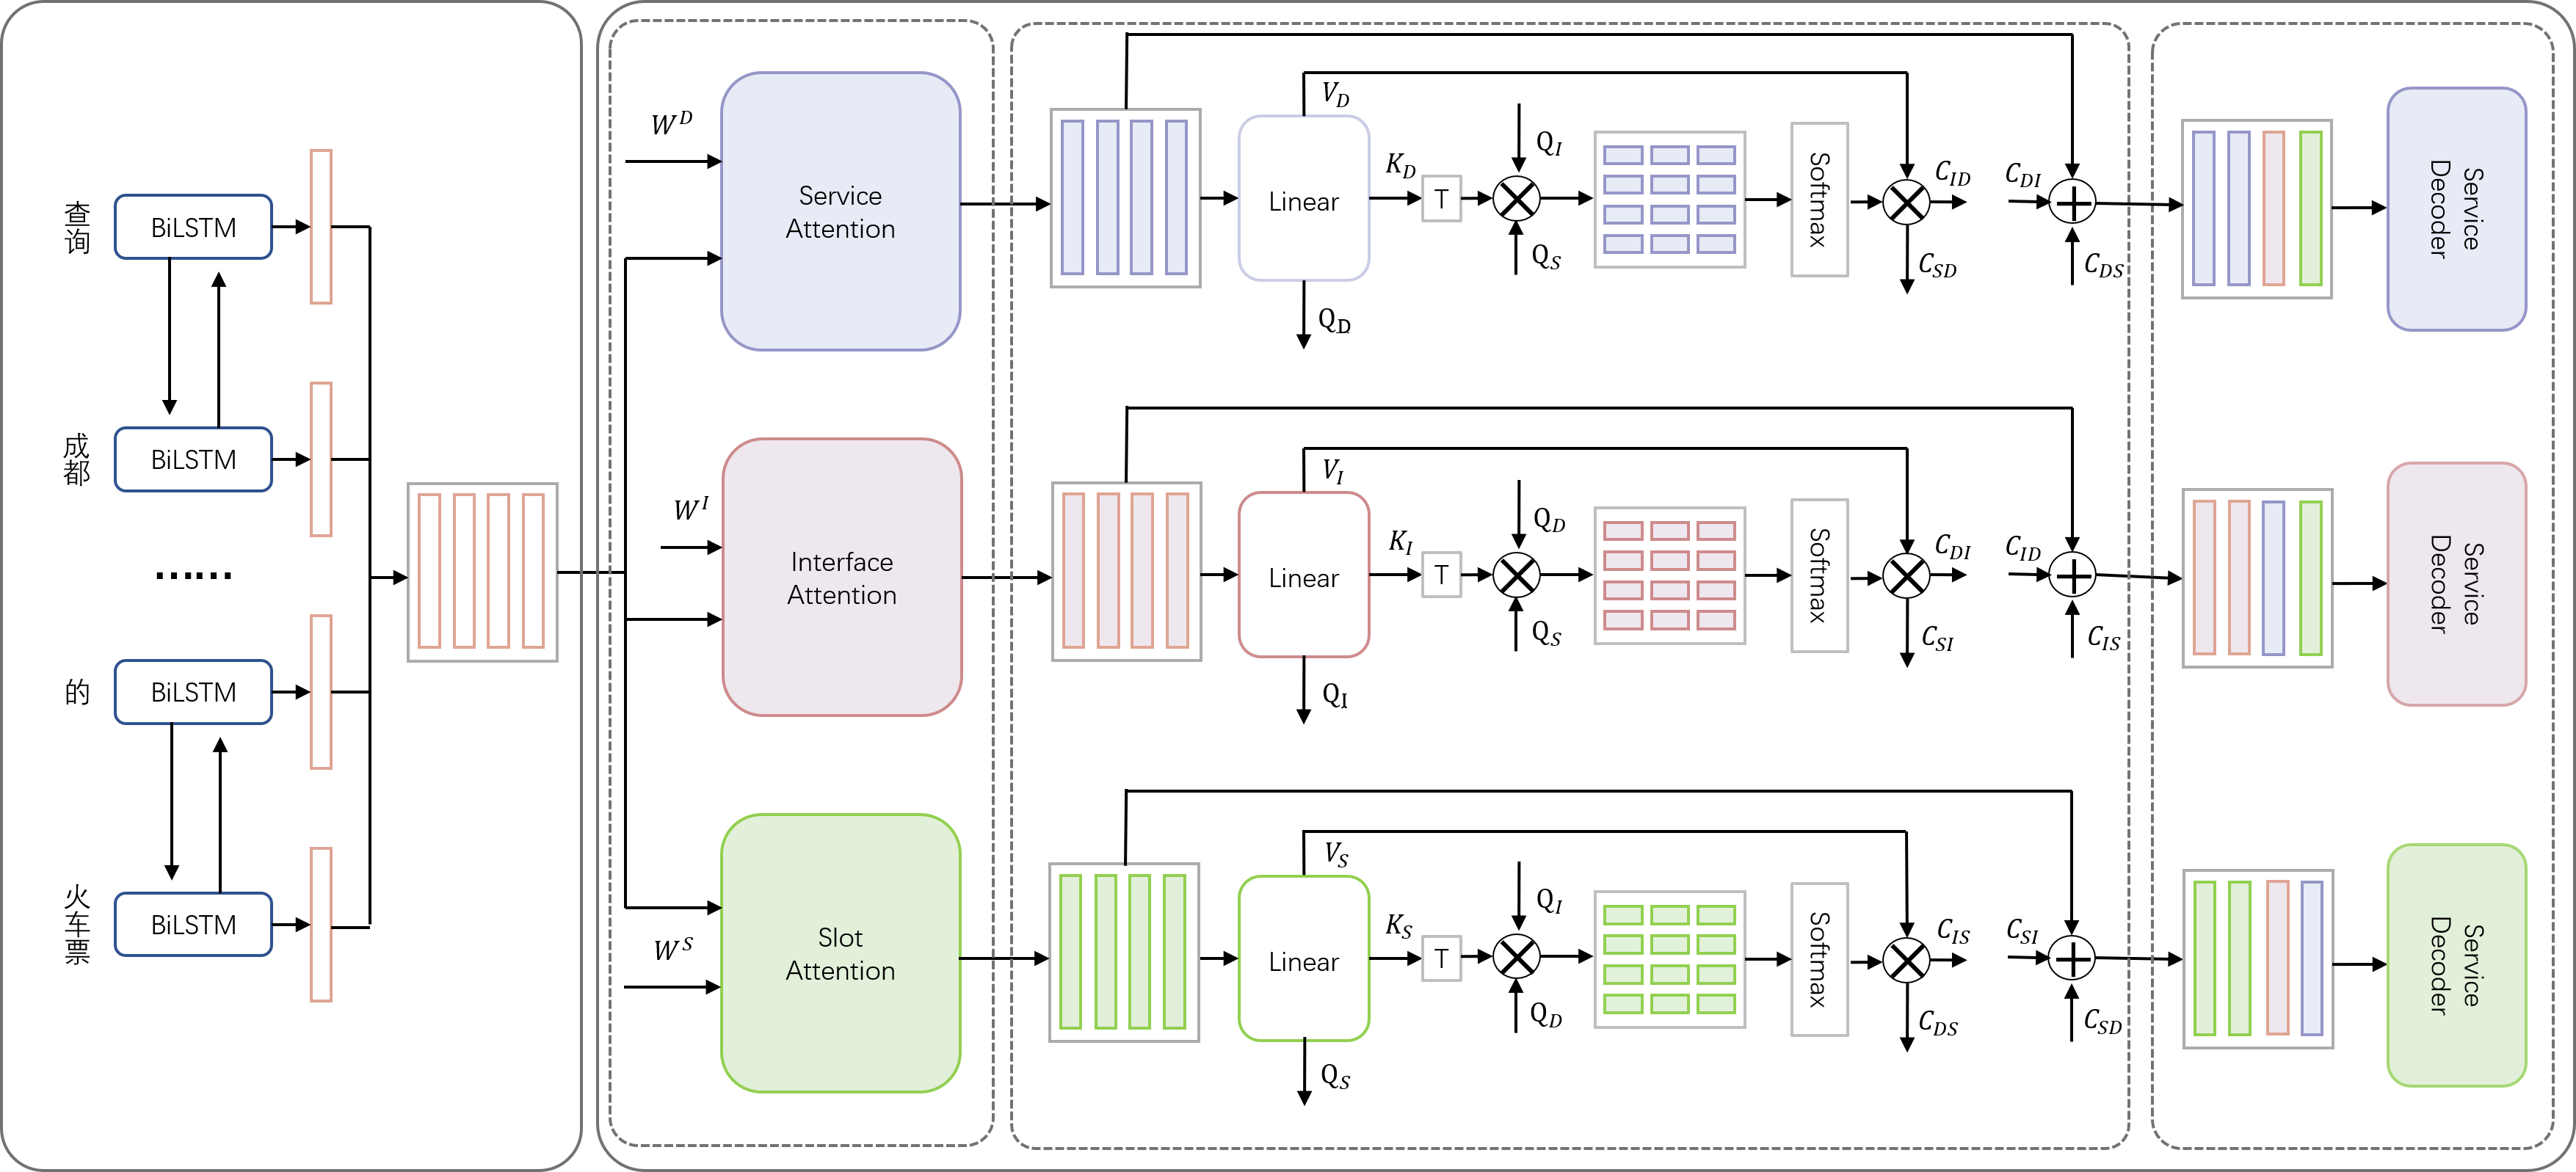
\includegraphics[width=16cm]{./images/co-interactive.jpg}
  \caption{交互式联合识别模型}
  \label{fig:lianhe2}
\end{figure}


交互式联合识别模型的结构如图\ref{fig:lianhe2}所示,主要包含的部分是:共享编码层,注意力层,协同交互层,独立解码层,接下将分别介绍:

(1)共享编码层

我们使用双向LSTM作为编码器,设输入词序列是x=[$x_{1}$,$x_{2}$,\dots,$x_{n}$](n为词的数量),$x_{i}$经过双向LSTM处理后
得到的结果是$\overleftarrow{\mathbf{h}}_{i}$和$\overrightarrow{\mathbf{h}}_{i}$,拼接以后在第i步得到的结果是$\mathbf{h}_{i}=[\overrightarrow{\mathbf{h}}_{i} ;\overleftarrow{\mathbf{h}}_{i}]$,
因此编码后得到的矩阵为$\mathbf{H}$=[$h_{1}$,$h_{2}$,\dots,$h_{n}$]。

(2)自注意力层

我们为服务分类、接口分类和参数填充三个任务分别引入了自注意力机制,将自注意力层处理以后得到的向量作为相应任务的矩阵表示传入协同交互层。
三者的attention原理相同,只是会训练各自的参数,因此可以合并介绍。
我们引入上下文向量${c}_{i}$来表示经过attention权重$α_{i,j}$处理后的BLSTM隐层向量:
\begin{equation}
    \mathbf{c}_{i}=\sum_{j=1}^{n} \alpha_{i, j} \mathbf{h}_{j}
  \end{equation}
  经过attention处理的句子矩阵表示为$\mathbf{C}$=[$c_{1}$,$c_{2}$,\dots,$c_{n}$],其中$\alpha_{i, j}$根据所在具体的attention层不同分为$\alpha_{i, j}^{D}$,$\alpha_{i, j}^{I}$,$\alpha_{i, j}^{S}$,计算公式如下:
  \begin{equation}
    \alpha_{t, j}=\frac{\exp \left(\operatorname{score}\left(\mathbf{h}_{i}, \mathbf{h}_{j}\right)\right)}{\sum_{k} \exp \left(\operatorname{score}\left(\mathbf{h}_{i}, \mathbf{x}_{k}\right)\right)}
    \end{equation}
    \begin{equation}
      \operatorname{score}(\mathbf{h}_{i}, \mathbf{h}_{j}))=\tanh \left(\mathbf{W}\left[\mathbf{h}_{i} ; \mathbf{h}_{j}\right]\right)
    \end{equation}
显然这里的$\mathbf{W}$根据任务不同分为$\mathbf{W}_D$,$\mathbf{W}_I$,$\mathbf{W}_S$,最后我们将H矩阵与attention处理的C矩阵相加:
\begin{equation}
  \mathbf{H}=\mathbf{H}+\mathbf{C}
\end{equation}
这里H根据训练时参数的不同分为三类$\mathbf{H}_{D},\mathbf{H}_{I},\mathbf{H}_{S}$,分别表示服务分类、接口分类向参数填充三项任务语义相关的显示的矩阵表示。

(3)协同交互层

本层是多个任务的信息流建立信息交换的核心层,上层共得到三个矩阵$\mathbf{H}_{D},\mathbf{H}_{I},\mathbf{H}_{S}$,他们是任务相关的独立的语义表示,本层主要目的
是在借助其他两项任务指导下更新当前任务对应的H矩阵,达到交互信息流的目的,提高模型准确率。
首先我们将$\mathbf{H}_{D},\mathbf{H}_{I},\mathbf{H}_{S}$分别做三组线性变换得到矩阵($\mathbf{Q}_{D},\mathbf{Q}_{I},\mathbf{Q}_{S}$),
($\mathbf{K}_{D},\mathbf{K}_{I},\mathbf{K}_{S}$),($\mathbf{V}_{D},\mathbf{V}_{I},\mathbf{V}_{S}$),之后的计算借鉴attention思想。
对于服务分类任务,将$\mathbf{Q}_{D}$做为queries,$\mathbf{K}_{I}$做为keys和$\mathbf{V}_{I}$做为values,$\mathbf{K}_{S}$做为keys和$\mathbf{V}_{S}$做为values,做以下处理来达到信息的交互:
\begin{equation}
  \mathbf{C}_{\mathbf{DI}}=\operatorname{softmax}\left(\frac{\mathbf{Q}_{\mathbf{D}} \mathbf{K}_{\mathbf{I}}^{\top}}{\sqrt{d_{k}}}\right) \mathbf{V}_{\mathbf{I}}\\
\end{equation}
\begin{equation}  
\mathbf{C}_{\mathbf{DS}}=\operatorname{softmax}\left(\frac{\mathbf{Q}_{\mathbf{D}} \mathbf{K}_{\mathbf{S}}^{\top}}{\sqrt{d_{k}}}\right) \mathbf{V}_{\mathbf{S}}\\
\end{equation}
\begin{equation}  
\mathbf{H}_\mathbf{D}=\mathbf{H}_\mathbf{D}+\mathbf{C}_{\mathbf{DI}}+\mathbf{C}_{\mathbf{DS}}
\end{equation}
对于接口分类任务,将$\mathbf{Q}_{I}$做为queries,$\mathbf{K}_{D}$做为keys和$\mathbf{V}_{D}$做为values,$\mathbf{K}_{S}$做为keys和$\mathbf{V}_{S}$做为values,做以下处理来达到信息的交互:
\begin{equation}
  \mathbf{C}_{\mathbf{ID}}=\operatorname{softmax}\left(\frac{\mathbf{Q}_{\mathbf{I}} \mathbf{K}_{\mathbf{D}}^{\top}}{\sqrt{d_{k}}}\right) \mathbf{V}_{\mathbf{D}}\\
\end{equation}
\begin{equation}
  \mathbf{C}_{\mathbf{IS}}=\operatorname{softmax}\left(\frac{\mathbf{Q}_{\mathbf{I}} \mathbf{K}_{\mathbf{S}}^{\top}}{\sqrt{d_{k}}}\right) \mathbf{V}_{\mathbf{S}}\\
\end{equation}
\begin{equation}
  \mathbf{H}_\mathbf{I}=\mathbf{H}_\mathbf{I}+\mathbf{C}_{\mathbf{ID}}+\mathbf{C}_{\mathbf{IS}}
\end{equation}
对于接口分类任务,将$\mathbf{Q}_{S}$做为queries,$\mathbf{K}_{D}$做为keys和$\mathbf{V}_{D}$做为values,$\mathbf{K}_{I}$做为keys和$\mathbf{V}_{I}$做为values,做以下处理来达到信息的交互:
\begin{equation}
  \mathbf{C}_{\mathbf{SD}}=\operatorname{softmax}\left(\frac{\mathbf{Q}_{\mathbf{S}} \mathbf{K}_{\mathbf{D}}^{\top}}{\sqrt{d_{k}}}\right) \mathbf{V}_{\mathbf{D}}\\
\end{equation}
\begin{equation}
  \mathbf{C}_{\mathbf{SI}}=\operatorname{softmax}\left(\frac{\mathbf{Q}_{\mathbf{S}} \mathbf{K}_{\mathbf{I}}^{\top}}{\sqrt{d_{k}}}\right) \mathbf{V}_{\mathbf{I}}\\
\end{equation}
\begin{equation}
  \mathbf{H}_\mathbf{S}=\mathbf{H}_\mathbf{S}+\mathbf{C}_{\mathbf{SD}}+\mathbf{C}_{\mathbf{SI}}
\end{equation}

其中$d_k$是Q,K矩阵的列数。我们认为经过上面计算更新过后的矩阵$\mathbf{H}_{D},\mathbf{H}_{I},\mathbf{H}_{S}$,包含了更丰富的语义信息,
实现了多任务之间信息的交互。
同时如图中标识(N×),N为超参数,协同交互层可堆叠在一起形成层次结构,使任务之间能够进行多次交互,实现增量捕获交互信息来达到彼此丰富。

(4)独立解码层

在经过共享的协同交互层以后,各任务拥有自己独立的解码层。
对于服务分类任务,我们使用上一章介绍的CNN的max-pooling方法,将$\mathbf{H}_{D}$经过max-pooling处理得到一个句子语义级表示的向量$\mathbf{M}_D$,
之后经过softmax函数:
\begin{equation}
  \mathbf{y}^{D}=\operatorname{softmax} (\mathbf{W}^{D}\mathbf{M}_D+\mathbf{b}^{D})
\end{equation}
\begin{equation}
  \mathbf{O}^{D}=\operatorname{argmax} (\mathbf{y}^{D})
\end{equation}
$\mathbf{y}^{D}$是输出的服务类别的分布,$\mathbf{O}^{D}$是预测的服务类别,$\mathbf{W}^{D}$和$\mathbf{b}^{D}$都是训练的参数。
对于接口分类任务解码器也做同样的处理,使用CNN的max-pooling方法,将$\mathbf{H}_{D}$经过max-pooling处理得到一个句子语义级表示的向量$\mathbf{M}_I$,
之后经过softmax函数:
\begin{equation}
  \mathbf{y}^{I}=\operatorname{softmax} (\mathbf{W}^{I}\mathbf{M}_I+\mathbf{b}^{I})
\end{equation}
\begin{equation}
  \mathbf{O}^{I}=\operatorname{argmax} (\mathbf{y}^{I})
\end{equation}
$\mathbf{y}^{I}$是输出的服务类别的分布,$\mathbf{O}^{I}$是预测的服务类别,$\mathbf{W}^{I}$和$\mathbf{b}^{I}$都是训练的参数。
对于参数提取即语义槽填充任务,为了更好的建模标签与标签之间的依赖性,我们在解码层加了CRF处理,如下式所示:
\begin{equation}
  \mathbf{O}_{\mathbf{S}} =\mathbf{W}^{\mathbf{S}} {\mathbf{H}}_{\mathbf{S}}+\mathbf{b}_{\mathbf{S}} 
\end{equation}
\begin{equation}
  P\left(\hat{\mathbf{y}} \mid \mathbf{O}_{\mathbf{S}}\right) =\frac{\sum_{i=1} \exp f\left(y_{i-1}, y_{i}, \mathbf{O}_{\mathbf{S}}\right)}{\sum_{y^{\prime}} \sum_{i=1} \exp f\left(y_{i-1}^{\prime}, y_{i}^{\prime}, \mathbf{O}_{\mathbf{S}}\right)}
  \end{equation}
  $f(y_{i-1}, y_{i}, \mathbf{O}_{\mathbf{S}})$表示从标签$y_{i-1}$到标签$y_{i}$的转移分数,以及标签$y_{i}$自身的得分。
同时我们采用联合损失函数的形式对三项任务一起训练,服务分类预测的交叉熵损失函数可记为:
\begin{equation}
\mathcal{L}_{1} \triangleq-\sum_{j=1}^{m} \hat{\mathbf{y}}^{j, \mathbf{D}} \log \left(\mathbf{y}^{j, \mathbf{D}}\right)
\end{equation}
同理,接口分类交叉熵损失函数可记为:
\begin{equation}
  \mathcal{L}_{2} \triangleq-\sum_{j=1}^{m} \hat{\mathbf{y}}^{j, \mathbf{I}} \log \left(\mathbf{y}^{j, \mathbf{I}}\right)
  \end{equation}
  参数语义槽填充交叉熵损失函数可记为:
  \begin{equation}
    \mathcal{L}_{3} \triangleq-\sum_{j=1}^{m} \sum_{i=1}^{n_{j}} \hat{\mathbf{y}}_{i}^{j, \mathbf{S}} \log \left(\mathbf{y}_{i}^{j, \mathbf{S}}\right)
  \end{equation}
  其中$\hat{\mathbf{y}}^{j, \mathbf{D}},\hat{\mathbf{y}}^{j, \mathbf{I}},\hat{\mathbf{y}}_{i}^{j, \mathbf{S}}$为真实值,m是训练的数据总量,联合损失函数
  可表示为:
  \begin{equation}
    \mathcal{L}_{\theta}=\alpha \mathcal{L}_{1}+\beta \mathcal{L}_{2}+(1-\alpha-\beta) \mathcal{L}_{3}
  \end{equation}
  其中$\alpha,\beta$为超参数。

\section{结合bert的模型}

大量研究表明,语言模型预训练对于学习通用语言表示很有用,作为最新的语言模型预训练模型,BERT在许多语言理解任务中均取得了惊人的成绩。
bert预训练模型的使用可以避免从头开始训练新模型,它通过利用大量非标注数据来学习语言的通用表示形式。

官方提供了不同参数的多版本bert供用户使用,本文从中选择的是BERT-Base Chinese,
其中核心参数 L = 12, H = 768, A = 12 ,params的总量为 110 M。具体来说, L = 12 指 Transformer 的层数为 12 层,
 H = 768 表示 Transformer 内部 包含 768 个隐含单元, A = 12 表示多头自制力机制中自注意力机制个数为 12 个\cite{devlin2018bert}。
 BERT依赖于Transformer,一个基本的Transformer由一个读取文本输入的编码器和一个对任务进行预测的解码器组成。
BERT编码器的输入是一系列token,这些token首先被转换为矢量,然后在神经网络中进行处理。
但是在开始处理之前,BERT需要对输入进行处理并用一些额外的元数据修饰:

1.令牌嵌入:在第一个句子的开头将[CLS]令牌添加到输入的单词令牌中,并在每个句子的末尾插入[SEP]令牌。

2.段嵌入:将指示输入属于句子A或句子B的标记添加到每个标记,这使编码器能够区分输入属于哪个句子。

3.位置嵌入:将位置嵌入添加到每个标记,以指示词在句子中的位置。

因此,引入bert模型以后我们不再需要结巴分词工具,直接将句子按字向量序列输入bert模型编码,bert对输入的处理如图\ref{fig:bertInput}。
\begin{figure}[htbp]
  \centering
  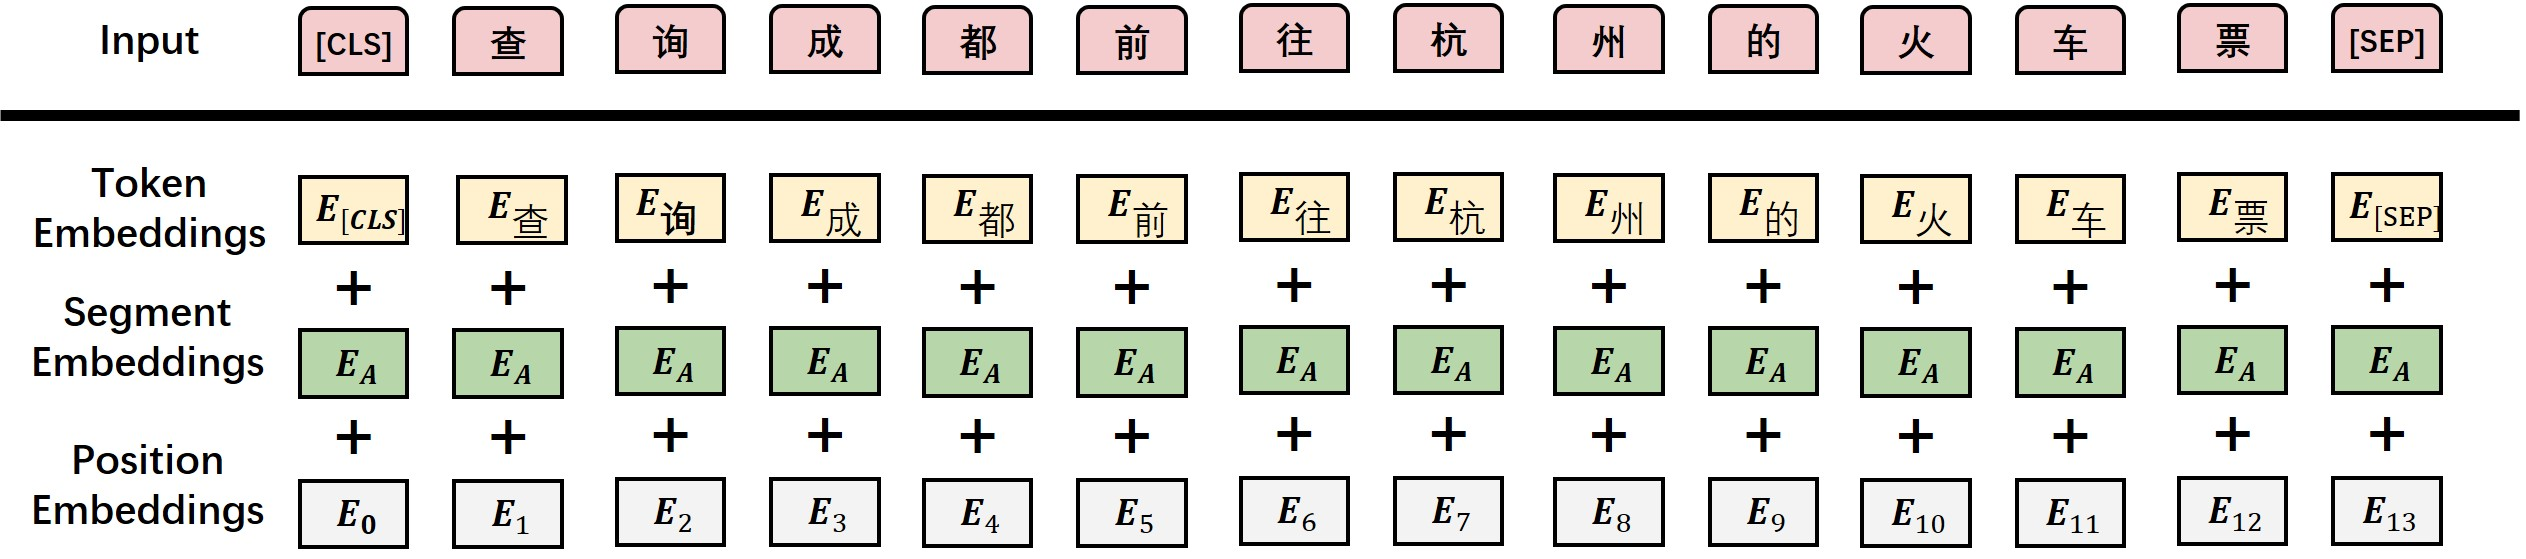
\includegraphics[width=18cm]{./images/bertInput.jpg}
  \caption{bert对输入的处理}
  \label{fig:bertInput}
\end{figure}

\subsection{bert-base联合识别模型}
首先,我们提出最简版的bert-base模型,
将服务分类、接口分类和参数填充三个任务利用联合损失函数隐式的建模,本模型主要起对照组的作用,
来验证引入bert是否能够给NLU带来增益,同时可以作为下一个模型的baseline,模型架构如图\ref{fig:bert-base}所示。

\begin{figure}[htbp]
  \centering
  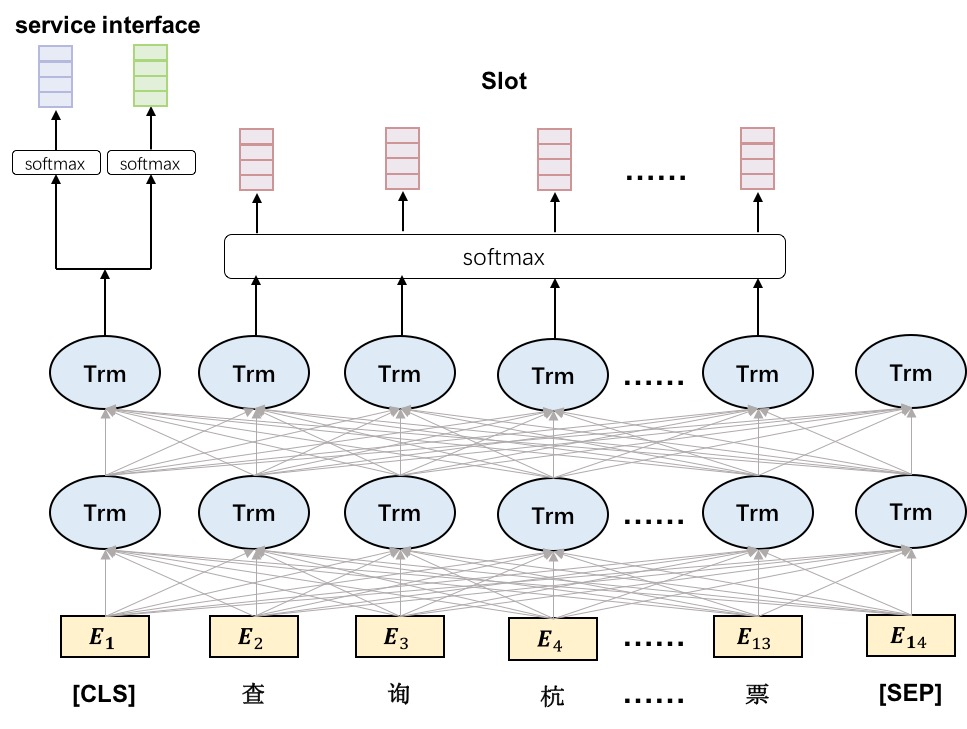
\includegraphics[width=15cm]{./images/bert-base.jpg}
  \caption{bert-base联合识别模型}
  \label{fig:bert-base}
\end{figure}

模型结构非常清晰,将用户语句按字向量序列输入bert模型编码,得到bert的输出$\mathbf{H}$=[$h_{1}$,$h_{2}$,\dots,$h_{n}$],
我们取bert输出的第一个向量,也就是特殊token([CLS])的隐藏状态作为两项分类任务的输入传给softmax层:
\begin{equation}
  y^{d}=\operatorname{softmax}\left(\mathbf{W}^{d} \boldsymbol{h}_{1}+\boldsymbol{b}^{d}\right)
\end{equation}
\begin{equation}
  y^{i}=\operatorname{softmax}\left(\mathbf{W}^{i} \boldsymbol{h}_{1}+\boldsymbol{b}^{i}\right)
\end{equation}
对于参数填充任务,将[$h_{2}$,\dots,$h_{n}$]隐层状态传入softmax层,以对插槽填充标签进行分类:
\begin{equation}
y_{n}^{s}=\operatorname{softmax}\left(\mathbf{W}^{s} \boldsymbol{h}_{n}+\boldsymbol{b}^{s}\right), n \in 2 \ldots N
\end{equation}
三项任务联合概率函数为:
\begin{equation}
  p\left(y^{d},y^{i}, y^{s} \mid \boldsymbol{x}\right)=p\left(y^{d} \mid \boldsymbol{x}\right) \left(y^{i} \mid \boldsymbol{x}\right) \prod_{n=1}^{N} p\left(y_{n}^{s} \mid \boldsymbol{x}\right)
  \end{equation}
  训练的目标是最大化正确标签的概率$p\left(y^{d},y^{i}, y^{s} \mid \boldsymbol{x}\right)$。

\subsection{bert-co-interactive联合识别模型}

为在co-interactive联合识别模型中引入bert,将其共享编码器换成bert拼接在attention层之前\ref{fig:bert-joint},模型其他结构与co-interactive模型
一致不再赘述,bert部分的参数采用fine-tuning的方式更新。
\begin{figure}[htbp]
  \centering
  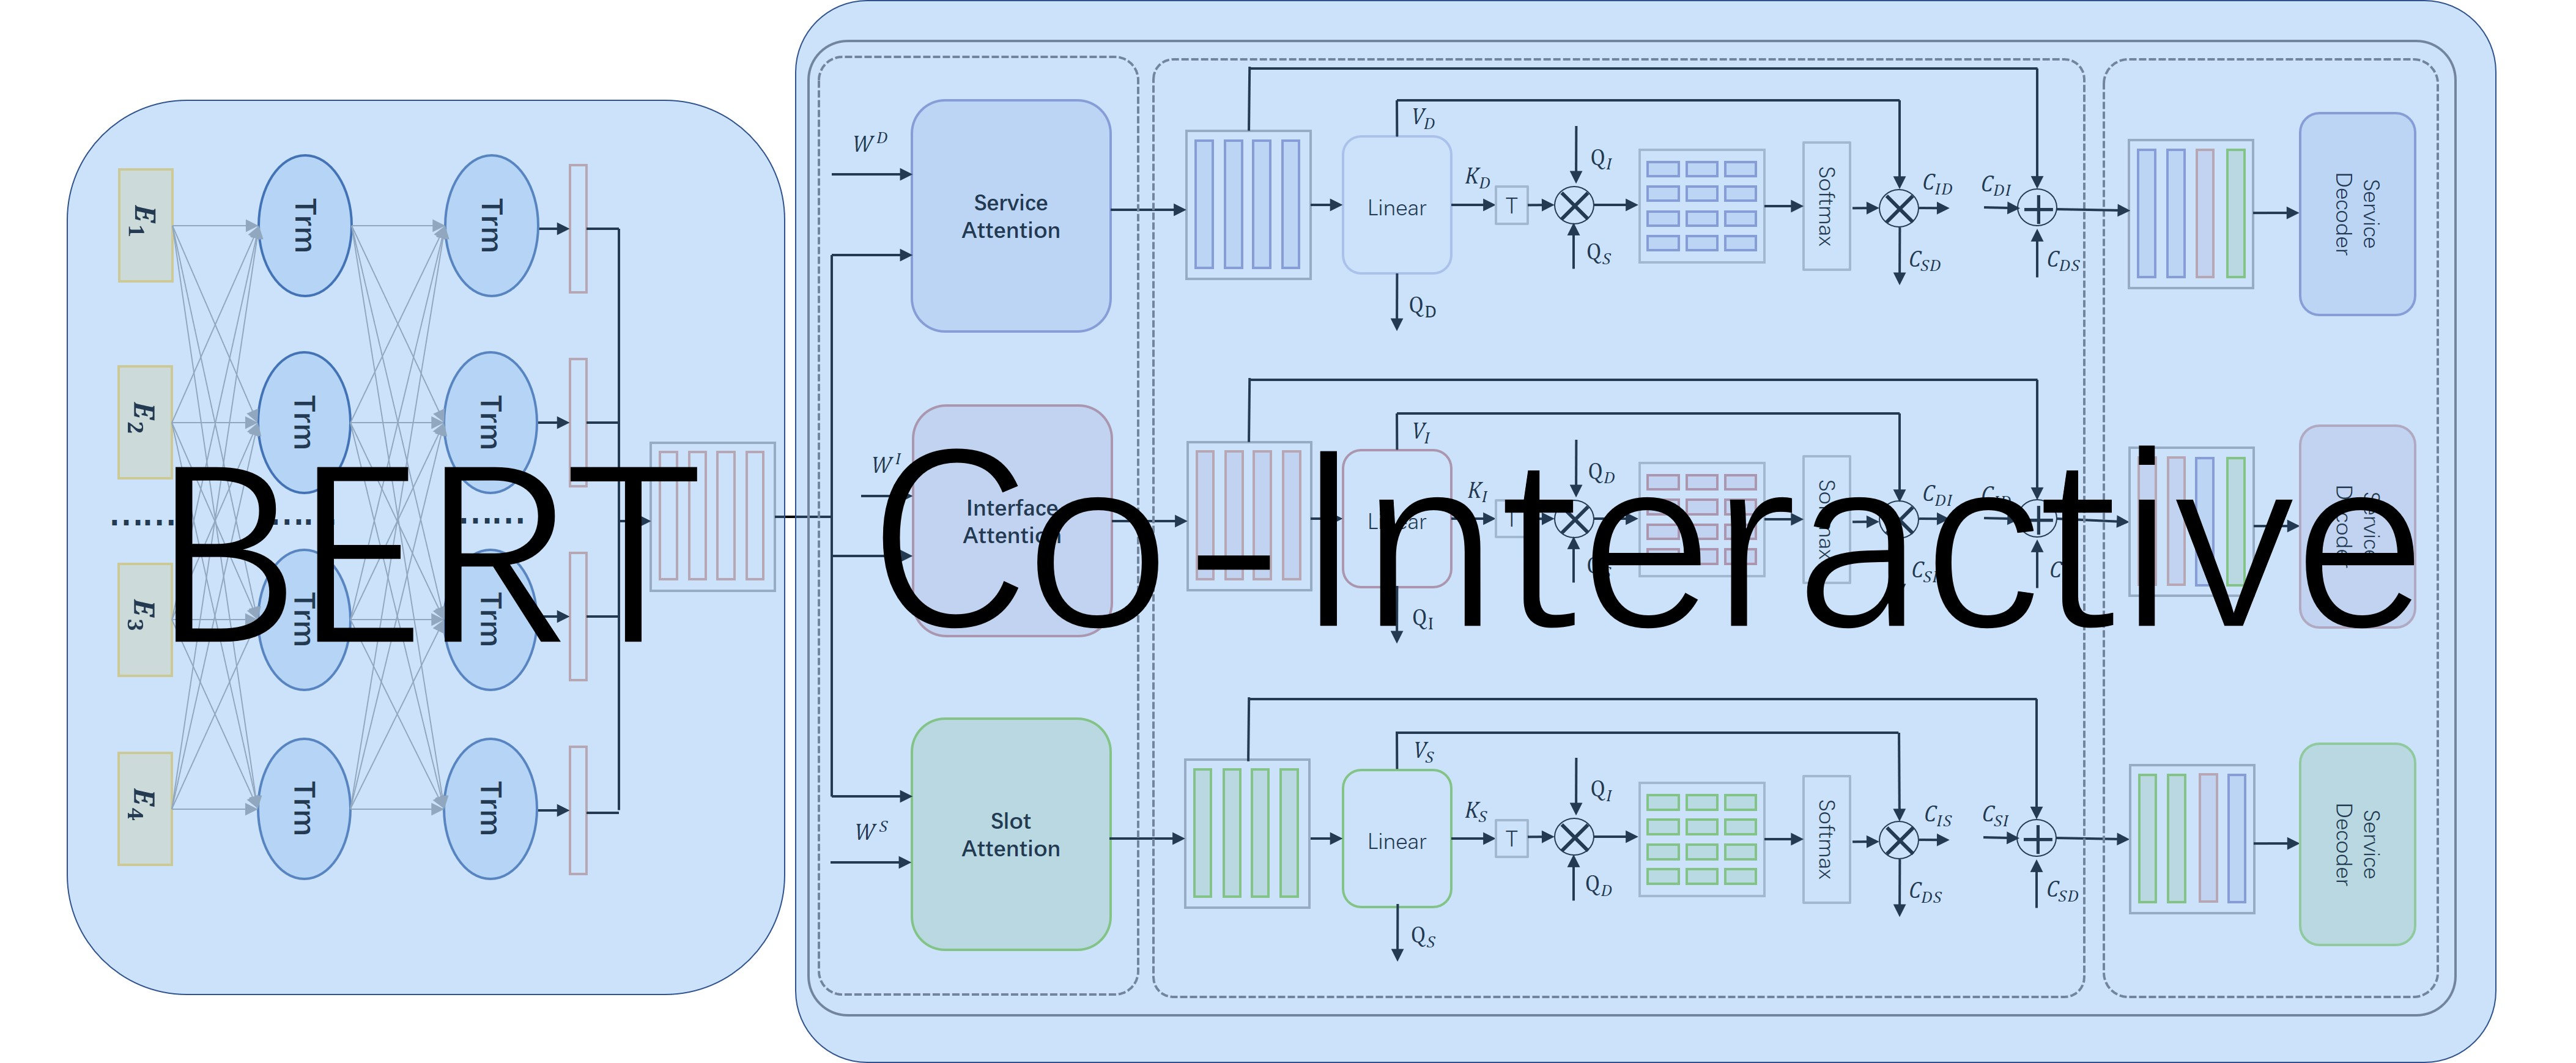
\includegraphics[width=14cm]{./images/bert-joint.jpg}
  \caption{引入bert交互式联合识别模型}
  \label{fig:bert-joint}
\end{figure}


% \section{结合ernie的模型}
\section{引入知识图谱}
与段落或文档不同,短文本输入做为信息源更加模糊,因为它们没有足够的上下文信息,这对语义理解造成了很大的挑战。
在本小节中,我们从外部知识源中检索知识,以增强短文本的语义表示。我们将概念性信息视为一种知识,并将其传入深度神经网络。
知识库(KB)中存在的重要语义关系,例如isA和isPropertyOf等,这些信息有助于理解短文本,尤其是模型在处理训练集中未出现的短语时。
例如,给定一个简短的文本“播放林俊杰的江南”,未引入KB的模型可能会将林俊杰当作普通人名,而无法学习到林俊杰是歌手,如果KB中林俊杰是歌手的知识
能输入到神经网络中,将有助于将文本归类于“music”服务。

如果将概念信息简单地集成到深度神经网络中,会存在一个问题:在概念化短文本时,由于实体的歧义或KB的噪声,很容易引入一些不正确或不想关的概念。
例如,在文本“查询苹果公司今日股价”,我们会从KB获得“苹果”的“水果”和“手机”概念。显然,这里的“水果”并不是一个恰当的概念,这是由实体的歧义造成的。
为了解决这个问题,衡量知识的重要性,我们使用C-T注意力(concept,text)来衡量短文本及其相应概念之间的语义相似性,
从而模型会将更大的权重分配给概念“手机”,因为它在语义上与短文本更接近,而不是概念“水果”。
借助概念性信息对短文本进行数据增强,与之前的方法不同,使模型像人类一样有了很多先验知识。如图\ref{fig:kg}所示,在bert-co-interactive联合识别模型
的基础上,本小节对其编码层进行了改进:
% 我们引入注意力机制,并提出了具有知识动力注意的深层短文本分类(STCKA)。

% 为了衡量知识的重要性,我们介绍了注意力机制,并提出了基于知识动力的注意力的短文本分类(STCKA),利用对短文本(CST)的关注和对概念集(C-CS)的关注来从两个方面获得概念的重要性。


% 我们借助诸如YAGO(Suchanek,Kasneci和Weikum 2008)和Freebase(Bollacker等人2008)之类的显式KB来丰富短文本的语义表示。
% 这允许模型从外部知识源检索知识,该知识未在短文本中明确说明,但与分类有关。如S1所示,作为一种知识的概念信息有助于分类。
% 因此,我们利用isA关系,并通过概念化1将每个短文本与其相关概念以KB关联。之后,我们将概念信息作为先验知识整合到深度神经网络中。


% 我们的模型包含四个模块。知识检索模块从知识库中检索与短文本相关的概念信息。
% 输入嵌入模块利用短文本的字符和单词级别功能来生成单词和概念的表示形式。
% 短文本编码模块通过自我注意对短文本进行编码,并产生短文本表示q。
% 知识编码模块对概念向量应用两种注意机制,以获得概念表示p。
% 接下来,我们将p和q连接起来以融合短文本和概念信息,这些信息将被馈送到完全连接的层中。
\begin{figure}[htbp]
  \centering
  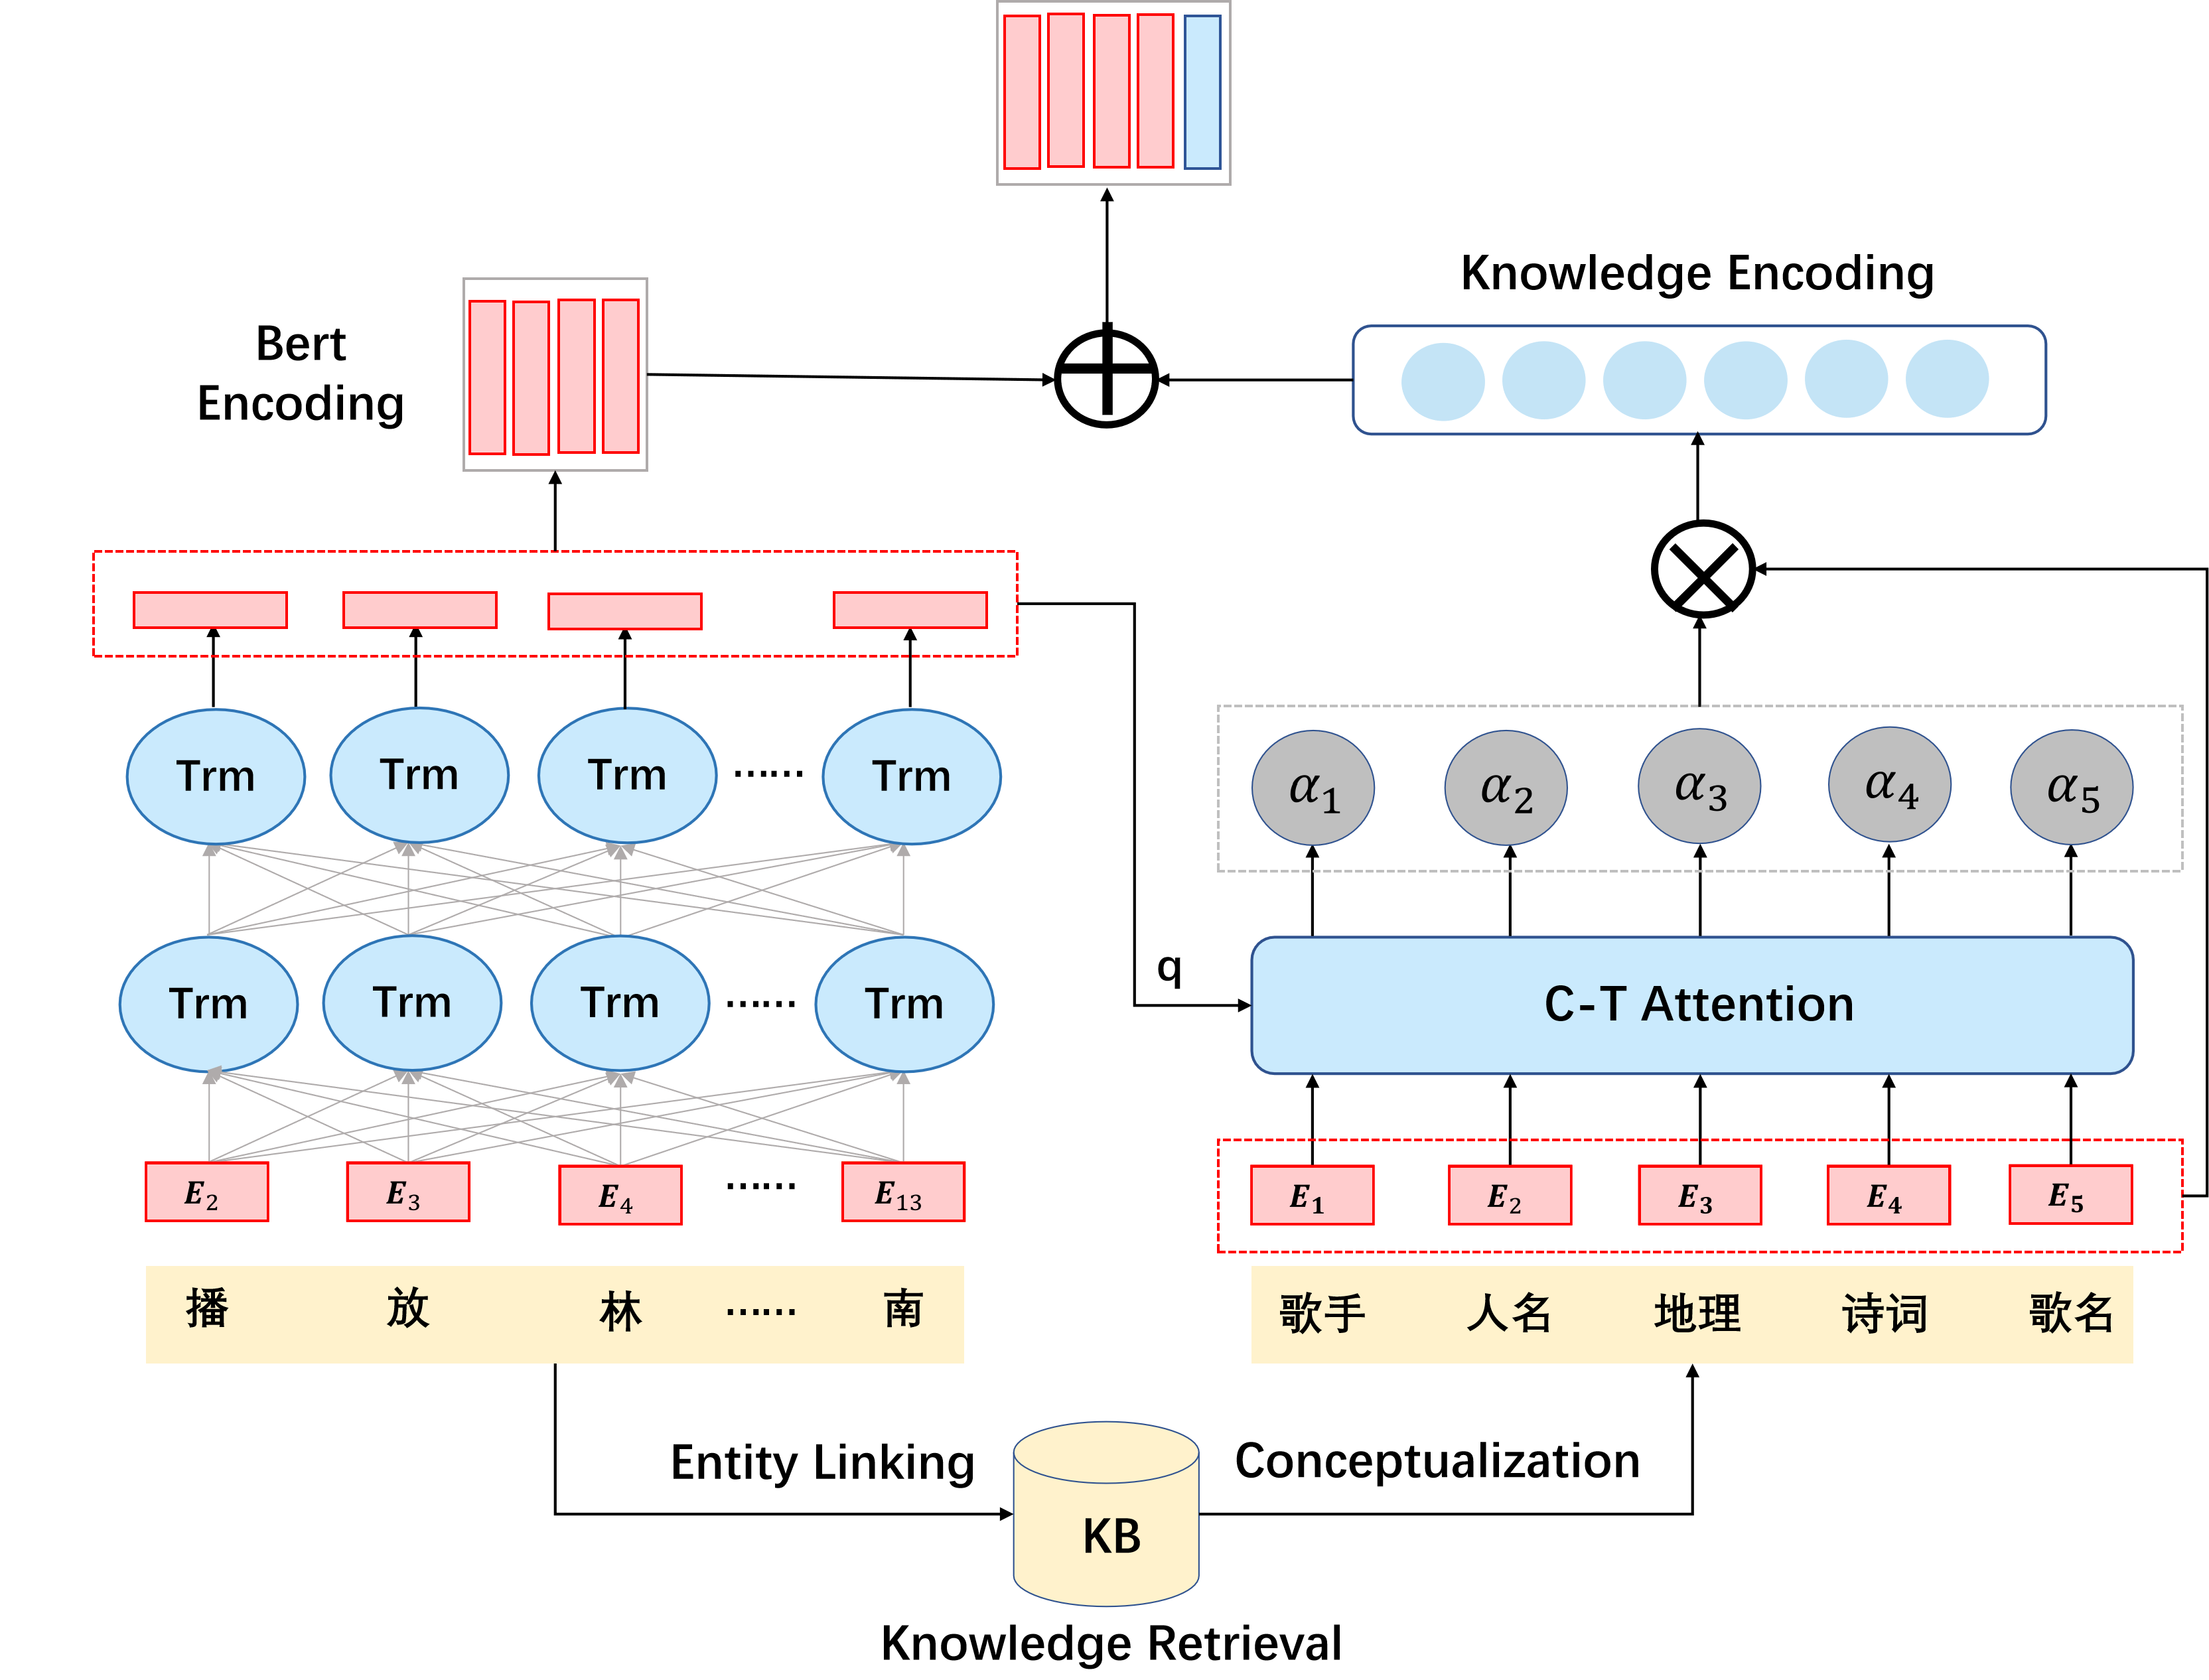
\includegraphics[width=16cm]{./images/kg.png}
  \caption{引入知识图谱的编码层}
  \label{fig:kg}
\end{figure}
(1)知识检索

该模块的目的是从知识库中检索相关知识,语义关系主要选用isA,isPropertyOf两种,给定一个简短的文本,希望找到与其相关的概念集C。
可通过两个主要步骤来实现此目的:实体链接和概念化。
实体链接是NLP中的一项重要任务,用于识别短文本中提到的实体\cite{moro2014entity},
本文通过利用现有的实体链接解决方案,获得了短文本的实体集E\cite{chen2018short}。
然后,对于每个实体e $\in$ E,我们通过概念化从CN-Probase现有知识库中获取其概念信息。
例如,给定一个用户输入文本“播放林俊杰的江南”,通过实体链接可获得实体集E = {林俊杰,江南}。
然后,我们将实体集E概念化,并从CN-Probase获得其概念集C = {人名,歌手,地理,诗词,歌名}。

(2)C-T attention
如前所述,简单地将所有概念信息集成到深度神经网络中,会存在实体的歧义或KB的噪声的问题,因此使用C-T注意力机制。
给定大小为m的概念集C,计为($c_1$,$c_2$,$\dots$,$c_m$),其中$c_i$是第i个概念向量,我们旨在产生概念集C的向量表示p。 
为了减少由于实体的歧义或KB噪声而引入的一些不正确概念,使用以下公式来计算C-T注意力以衡量第i个概念与文本表示向量q之间的语义相似性:
\begin{equation}
\alpha_{i}=\operatorname{softmax}\left(w_{1}^{T} f\left(W\left[c_{i} ; q\right]+b\right)\right)
\end{equation}
其中q是bert输出的矩阵经过max-pooling处理得到的用户输入语句向量级表示,
$\alpha_{i}$表示第i个概念到短文本的注意权重,较大的$\alpha_{i}$表示第i个概念在语义上与短文本更相似,
f采用非线性激活函数双曲线正切变换,W和b是训练参数。
\begin{equation}
p=\sum_{i=1}^{m} a_{i} c_{i}
\end{equation}
最后通过加权求和得到knowledge encoding的向量表示p,将p和bert输出的矩阵连接得到引入知识的编码结果,
后续会传入co-interactive层,其结构已经在之前介绍过,不再赘述。

\section{本章小结}
本章利用任务之间存在的强关联性,将服务分类、接口分类和参数填充三项任务做了联合识别,包括单向信息流的联合和交互式联合两种尝试,
同时引入预训练模型bert对模型进行优化,在此基础上引入知识库丰富输入语句的语义信息,得到了不错的效果。
